\documentclass{scrartcl}
\usepackage{german}
\usepackage[utf8]{inputenc}
\usepackage[german]{babel}

% zusätzliche mathematische Symbole, AMS=American Mathematical Society
\usepackage{amssymb}
\usepackage{amsmath}
% fürs Einbinden von Graphiken
\usepackage{graphicx}

% für Namen etc. in Kopf- oder Fußzeile
\usepackage{fancyhdr}

% erlaubt benutzerdefinierte Kopfzeilen
\pagestyle{fancy}

% used for drawing the gantt-diagram
\usepackage{pgfgantt}


% Definition der Kopfzeile
\lhead{
\begin{tabular}{lllll}
Nils Hagner & 4346038 & Felix Karg & 4342014 \\
Michael Fleig & 4340085 & Anush Davtyan &4368689
\end{tabular}
}
\chead{}
\rhead{\today{}}
\lfoot{}
\cfoot{Seite \thepage}
\rfoot{}

\begin{document}

\section*{Solutions for Excercise sheet 2}

\subsection*{Exercise 1 – Cost Estimation}
\begin{itemize}
	\item[i]
	The resulting amount should be $30h*6=180h$ per person, and with $1 PM=20*8=160h$ it amounts to $6.75$ PMs or with five persons to $5.625$ PMs.\\
	\item[ii]
	\begin{tabular} {| c | c |}
		round & estimations ($KLOC_{pars}$)\\
		\hline
		0 & 10, 15, 14, 15 \\
		1 & 12, 13, 12, 10\\
		2 & 12\\
	\end{tabular}\\\\
	% TODO: Nils
	\item[iii]
	We decided for small size, greater innovation, medium deadlines and stable development environment. Because of this we chose a medium project with $a=3.0$ and $b=1.12$.\\
	\item[iv]
		\item[]Required software reliability: nominal
		\item[]Size of application database:  none
		\item[]Complexity of the product:  nominal
		\item[]Run-time performance constraints:   nominal
		\item[]Memory constraints:  nominal
		\item[]Volatility of the virtual machine env.:  none
		\item[]Computer turnaround time:  low
		\item[]Analyst capability:  low
		\item[]Applications experience:  low
		\item[]Software engineer capability:  nominal
		\item[]Virtual machine experience:  high
		\item[]Programming language experience:  very low
		\item[]Use of modern programming practices:  low
		\item[]Use of software tools:  nominal
		\item[]Required development schedule:  nominal


	\item[v]
	\begin{tabular}{l | c}
		parameter & chosen value \\
		\hline
		% Required software reliability: if the system fails, the user can loose all points achieved in the game, but the points can be achieved again in not a very long time.
		Required software reliability & 1\\
		% Size of application database: it is very low, we do not need a database.
		Size of application database & -\\
		% Complexity of a product: it is nominal, because: only standart math will be used; mostly simple nesting; some divice-dependent operations, like error prosessing, but no operations at the physical I/O level; only simple structural changes and simple edits.
		Complexity of the product & 1\\
		% Run-time performance constraints: nominal, because the software is processor-intensive.
		Run-time performance constraints  & 1\\
		% Memory constraints: nominal, because the group has only little experience, and we assume the program will be not very effective.
		Memory constraints & 1\\
		% Volatility: very low, no changes of the working environment.
		Volatility of the virtual machine env. & -\\
		% Computer turnaround time: low, the game is interactive.
		Computer turnaround time & 0.87\\
		% Analyst capability: low, too little experience.
		Analyst capability & 1.19\\
		% Applications experience: low, students do not have a lot of experience.
		Applications experience & 1.13\\
		% Software engineer capability: nominal, the developers should have some experience in teamwork.
		Software engineer capability & 1\\
		% Virtual machine experience: high, because the software(game) developing do not require very high virtual machine experience.
		Virtual machine experience & 0.9\\
		% Programming language experience: very low, almost no experience in C# or F#.
		Programming language experience & 1.14\\
		% Use of moderm programming practices: low, the group the group is only starting to use such practices.
		Use of modern programming practices & 1.1\\
		% Use of software tools: nominal, some useful software tools will be used.
		Use of software tools & 1\\
		% Required developemnt schedule: nominal, have a set deadline.
		Required development schedule & 1\\
	\end{tabular}\\\\
	The resulting project size in PM is (with $a=3$ and $b=1.12$):
	\[3 \cdot (12)^{1.12}\cdot (1\cdot 1 \cdot 1 \cdot 1 \cdot 0.87 \cdot 1.19 \cdot 1.13 \cdot 1 \cdot 0.9 \cdot 1.14 \cdot 1.1 \cdot 1 \cdot 1) \approx 64\]
	The two values differ drastically, the first is nearly a tenth of the second.
        This might be due to the way higher expectations of Code Quality or Project length, as well as the larger growth of smaller projects.
\end{itemize}

\subsection*{Exercise 2 – Process Modeling}

\begin{itemize}
    \item[i] Process model: \\ 
    	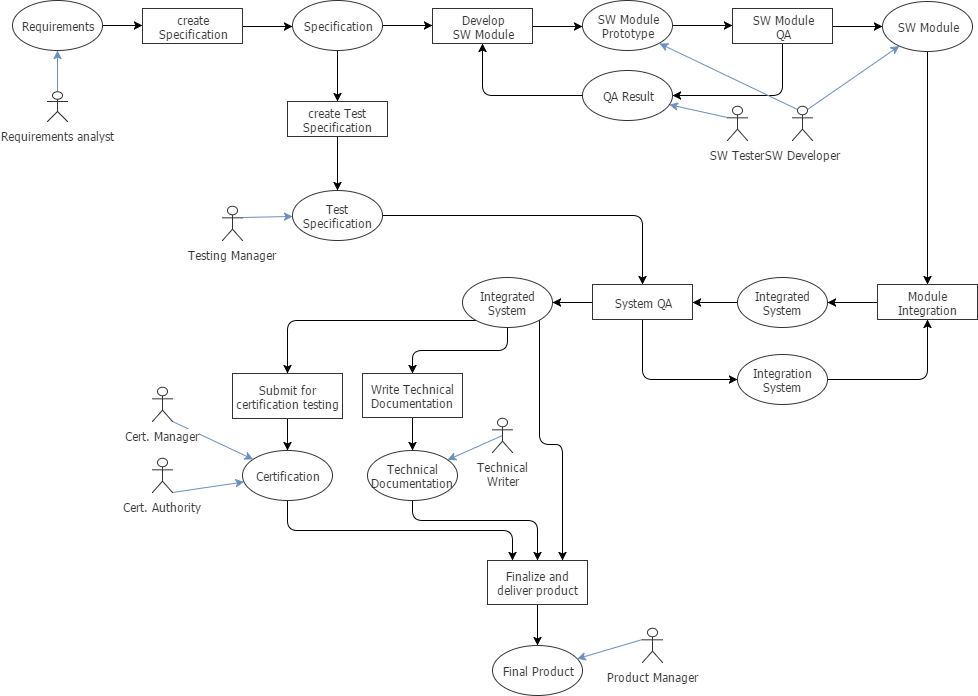
\includegraphics[width=\textwidth]{swt_2_1.png}
    \item[ii] (Might be on next page)
        % \documentclass{article}

% \usepackage{pgfgantt}

% \begin{document}


\begin{ganttchart}[
        hgrid,
        vgrid
    ]{1}{17}
    \gantttitle{Half Person-Months}{17} \\
    \gantttitlelist{1,...,17}{1} \\

    \ganttgroup{Maria}{1}{1}
    \ganttgroup{Maria}{11}{11} \\

    \ganttbar{Create Spec}{1}{1} \\

    \ganttgroup{Herbert}{2}{10} \\

    \ganttbar{SW Module Dev}{2}{4} \\
    \ganttbar{SW Module QA}{5}{6} \\
    \ganttbar{Module Integration}{7}{8} \\
    \ganttbar{System QA}{9}{10} \\
    \ganttbar{Create Test Spec}{11}{11} \\

    \ganttgroup{Karin}{12}{15} \\

    \ganttbar{Submit for cert Test}{12}{13} \\
    \ganttbar{Documentation}{14}{15} \\

    \ganttgroup{Jane}{16}{17} \\

    \ganttbar{Deliver}{16}{17}

\end{ganttchart} \\

I'm afraid to say that we were not capable of numbering through
correctly (in half PM's) or to correctly \LaTeX  quarter-PM's.
The used package seems to be not capable of doing so.

% \end{document}

    \item[iii] Process model with fire detector\\
    	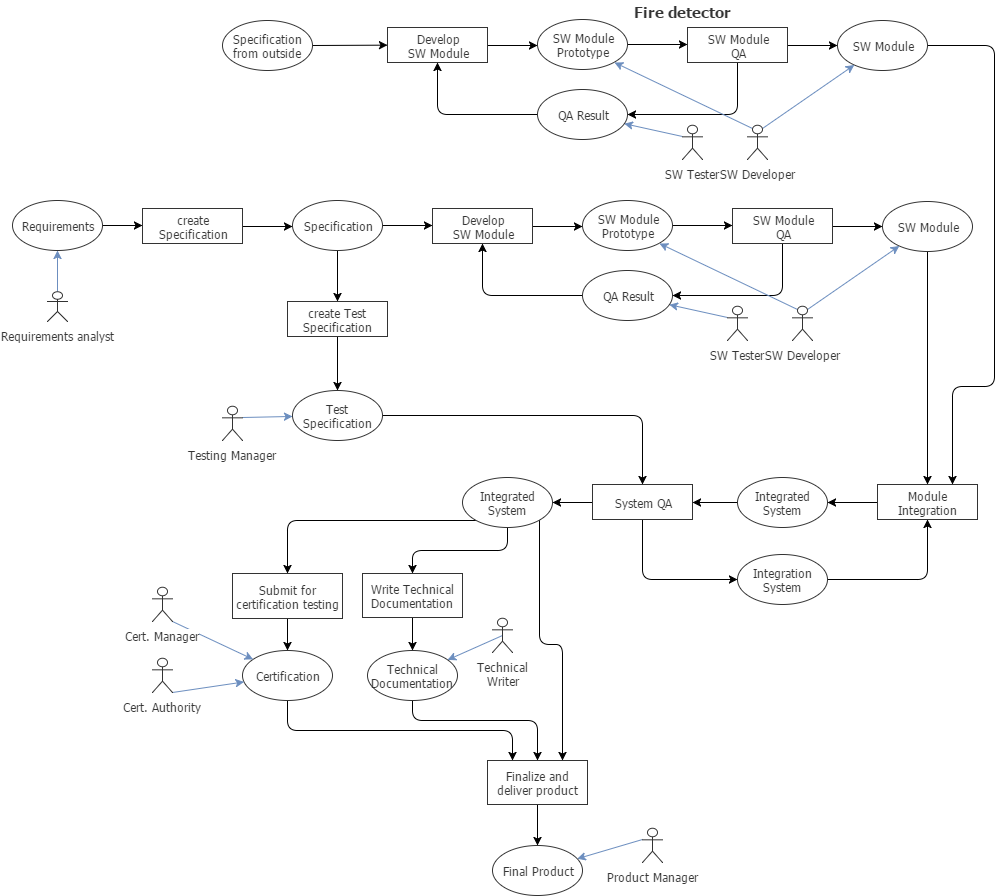
\includegraphics[width=\textwidth]{swt_2_3.png}
    \item[iv] Effort: 7.5 PM, minimum excpeted duration: 7.5 M
\end{itemize}

\end{document}
